\begin{frame}
\frametitle{Open Shop}
\begin{columns}
  \begin{column}{0.5\textwidth}
    \begin{center}
    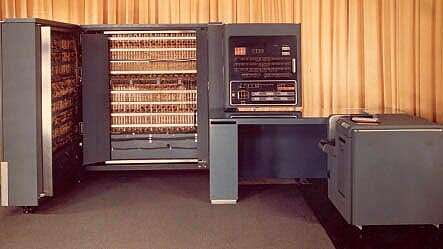
\includegraphics[width=\textwidth]{ibm701.jpg}
    \end{center}
  \end{column}
  \begin{column}{0.5\textwidth}
    \begin{itemize}
      \item IBM 701 - первый коммерческий компьютер от IBM;
      \item одна машина стоила \$2 млн. (50-ые)\footnotemark[1];
      \item месячная аренда ~15 000;
      \item из 15 минут работы - 10 настройка, и 5 вычисления;
    \end{itemize}
  \end{column}
\end{columns}
\footnotetext[1]{http://motherboard.vice.com/blog/the-rise-of-ibm-s-immortal-mainframe}
\end{frame}

\begin{frame}
\frametitle{Пакетная обработка}
\begin{columns}
  \begin{column}{0.5\textwidth}
    \begin{itemize}
      \item Человек - слабое звено, удалить человека!
      \item Машина сама может планировать задачи;
      \item основной критерий - уменьшение времени простоя;
      \item отдаете программу оператору, а потом пару дней ждете результата.
    \end{itemize}
  \end{column}
  \begin{column}{0.5\textwidth}
    \begin{center}
    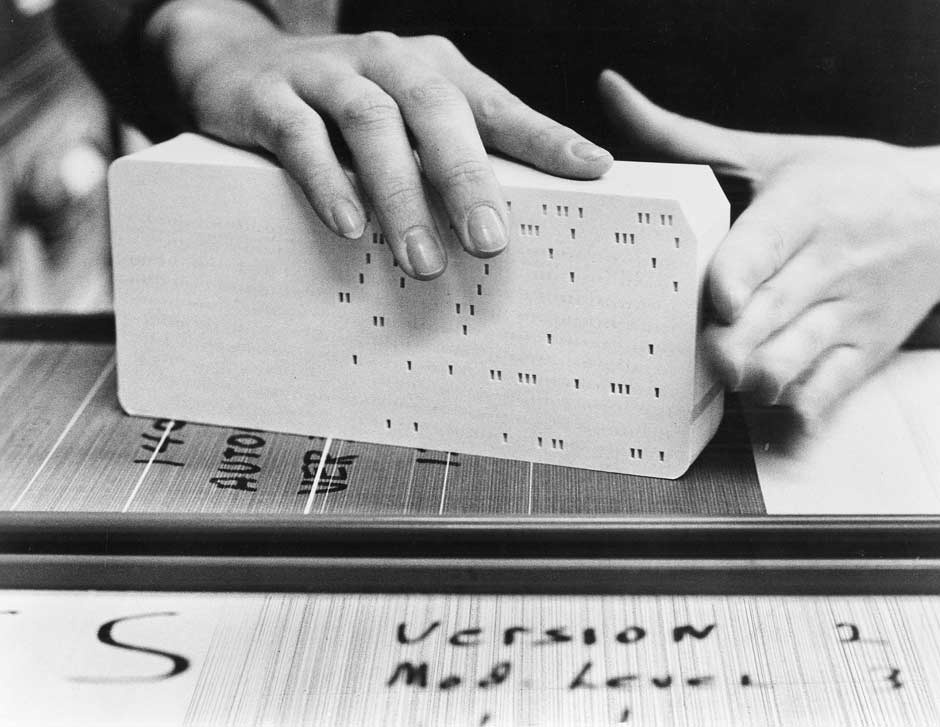
\includegraphics[width=\textwidth]{punched_card.jpg}
    \end{center}
  \end{column}
\end{columns}
\end{frame}

\begin{frame}
\frametitle{Многозадачность (Multiprogramming)}
\begin{itemize}
  \item Больше оперативной памяти - больше можно потратить на ерунду;
  \item энергонезависимая память произвольного доступа - нет строгой
  необходимости обрабатывать все последовательно;
  \item аппаратные прерывания позволяют выполнять ввод/вывод паралельно с
  расчетами и симулировать конкуретное исполнение (но об этом далее);
  \item примеры: B5000 MCP (60-ые, первая известная мне система с виртуальной
  памятью), Exec II (60-ые, позволяла засылать задачи удаленно, по телефону);
\end{itemize}
\end{frame}

\begin{frame}
\frametitle{Разделение времени}
\begin{itemize}
  \item Когда компьютеры становятся мощнее, инженеры начинают распускать руки;
  \item компьютерное время становится дешевле
  \begin{itemize}
    \item ждать пару дней завершения задачи на 5 мину - не целесообразно;
    \item хочется больше интерактивности - все пользователи получают свою долю;
  \end{itemize}
  \item примеры: CTSS (считается первой системой с разделением времени),
  Multics (академическое достижение и инженерный провал);
\end{itemize}
\end{frame}

\begin{frame}
\frametitle{Unix}
\begin{itemize}
  \item После провала Multics инженеры из Bell Labs стали искать альтернативы:
  \begin{itemize}
    \item Multics была слишком сложной поэтому проект и провалился;
    \item создатели Unix руководствовались простотой и проект взлетел;
    \item есть мнение, что популярность Unix стала препядствием для ее
    дальнейшего развития;
  \end{itemize}
\end{itemize}
\end{frame}

\begin{frame}
\frametitle{Concurrent Programming}
\begin{itemize}
  \item В начале 60-ых конкурентное исполнение уже существовало, а понимания как
  с ним работать правильно нет:
  \begin{itemize}
    \item первый систематический подход к созданию ОС был продемонстрирован
    Дейкстрой в его "THE multiprogramming system";
    \item Дейкстра же предложил концепцию семафора, как примитива синхронизации
    и взаимодействия;
    \item другим пример систематичного подхода к дизайну ОС стала RC 4000.
  \end{itemize}
\end{itemize}
\end{frame}

\begin{frame}
\frametitle{Personal Computers}
\begin{columns}
  \begin{column}{0.45\textwidth}
    \begin{center}
    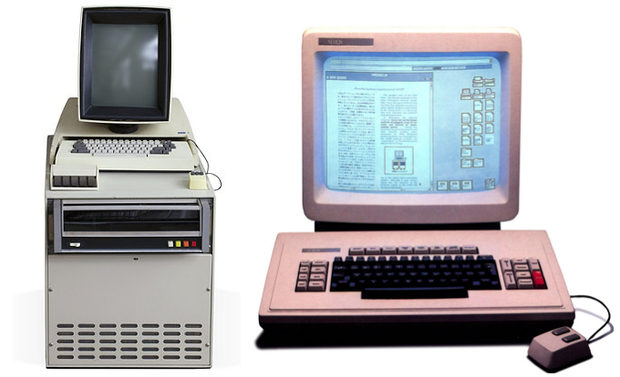
\includegraphics[width=\textwidth]{alto_star.png}
    \end{center}
  \end{column}
  \begin{column}{0.55\textwidth}
    \begin{itemize}
      \item 20 лет работы насмарку, ОС системы вновь стали:
      \begin{itemize}
        \item однопользовательскими;
        \item однопроцессными;
        \item простыми;
      \end{itemize}
      \item зато появился графический интерфейс и компьютерная мышь.
    \end{itemize}
  \end{column}
\end{columns}
\end{frame}
